\section{Implementation}
\label{sec:implementation}

The implementation was designed for use with the \ac{MPI} C library.  We use the \ac{GSL}
for the intra-processor linear algebra routines: primarily for computing dot products and
Mahalanobis distances.  PETSc handled inter-processor linear algebra, such as multiplying
$\mat{C}_N$ by another vector.  The code was compiled and tested on the \texttt{flux} CAEN
cluster.

We intended to use this project's code on the PCS shared-memory cluster to gauge how well
the code scales with many processors.  However, our code does not compile on
\texttt{blacklight} because the pre-installed PETSc version is quite old.  We therefore
only show results from the \texttt{flux} CAEN cluster, which has a recent release of
PETSc.

% Our initial impelementation used Cholesky decomposition on a shared memory PC with an
% NVIDIA GPU.  However, as mentioned above, Cholesky decomposition only works for relatively
% small matrices, and for 10,000-point datasets the execution times were unreasonable and we
% omit those results for this project.  As discussed in the following sections, a sparse
% iterative solver scales well and gives results in reasonable execution times.

\subsection{Partitioning the Covariance Matrix Between \acp{PE}}
\label{sub:partitioningthecovariancematrix}

For our implementation of the parallel \ac{GP}, each \ac{PE} owned the same area in the
covariance and \ac{RHS} vectors.  Figure~\ref{fig:partition} shows an example when $p$,
the number of \acp{PE}, is three.  This partitioning scheme could easily be acheived from
the \texttt{VecSetSizes()} and \texttt{MatSetSizes()} \ac{PETSc} routines.  By default,
these routines partition the processors as is shown in Figure~\ref{fig:partition}, however
other topologies are possible.

\begin{figure}[t]
  \begin{center}
    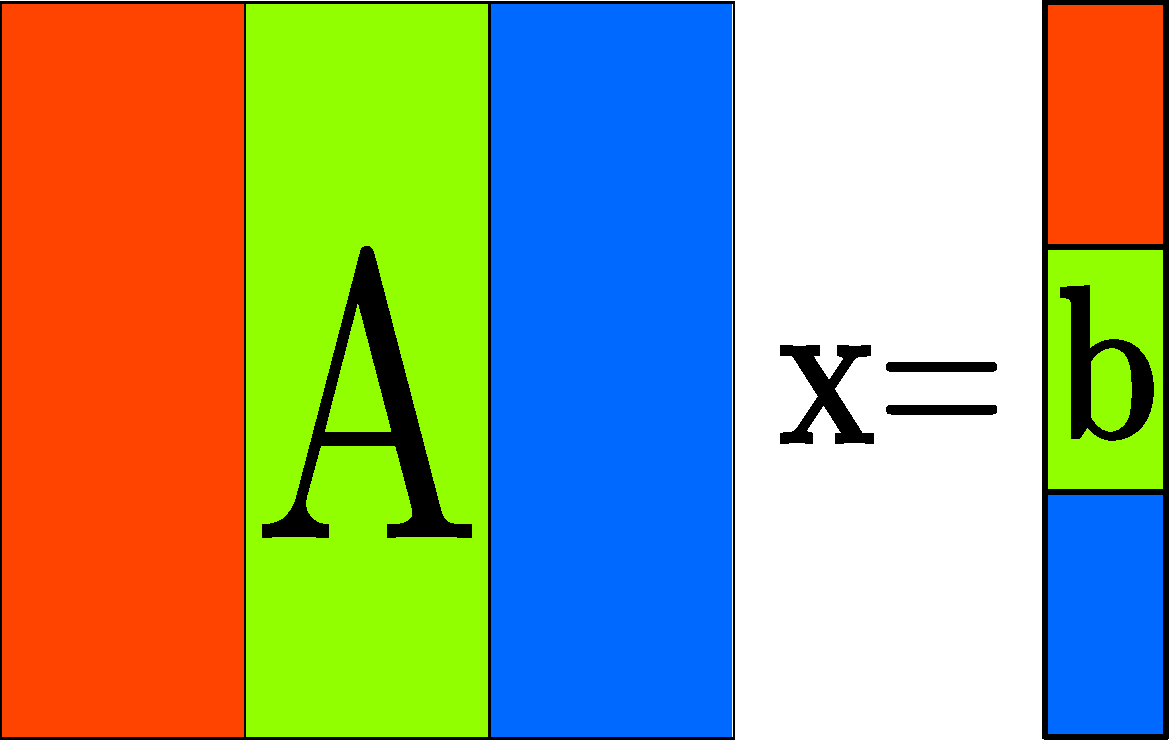
\includegraphics[width=.4\textwidth]{figures/columns}
    \caption{
      {\small 
        Example of how the linear system $\mat{A}{\bf x} = {\bf b}$ was partitioned
        for $p = 3$.  Each processor ``owned'' the same number of entries in the
        \ac{RHS} vector and covariance matrix.  The region corresponding to each processor
        is denoted by the separately colored regions.
      }
    }
    \label{fig:partition}
  \end{center}
\end{figure}

\subsection{Computing the Covariance Matrix and the Kernel Gradient}

Computing the covariance matrix and gradient is perhaps the most straightforward aspect of
this problem because every element in these matrices can be computed independently.
Furthermore, because $k({\bf x}, {\bf x}') = k({\bf x}', {\bf x})$, only the top-half of
the covariance matrix needs to be computed.  However, it is actually faster to have each
\ac{PE} compute its own elements rather than communicate its values to other processors.
Synchronizing the covariance matrix between all the \acp{PE} is conveniently handled by
PETSc.

\subsection{Solving $\mat{C}_N {\bf x} = {\bf b}$}
\label{sub:solving}

Solving for the vector ${\bf x}$ that satisfies $\mat{C}_N {\bf x} = {\bf b}$ for some
vector ${\bf b}$ is fairly straightforward with the help of PETSc.  In constructing the
iterative solver, we use the conjugate gradient method shown in Figure~\ref{fig:cg}.  For
the preconditioner, we use the Jacobi method because the diagonal elements of $\mat{C}_N$
are dominant.  This is simply because the kernel is maximal for any pair of training
points when the two training points are equal.

\subsection{Computing $\text{trace}\left(\mat{C}_{N}^{-1} \frac{\partial
      \mat{C}_N}{\partial {\boldsymbol \Theta}_i}\right)$}
\label{sub:trace}

Our method of computing the trace from Equation~\ref{eqn:learn} involves looping over the
columns of the gradient and solving a linear system with a \ac{KSP} solver (specifically,
one using the conjugate gradient method with a Jacobi preconditioner).  Each processor
keeps the trace of the portion of $C_N$ its assigned.  Finally, these sub-traces are
broadcast so every \ac{PE} has a vector of every other processor's sub-trace.  The trace
of the entire matrix is then simply the sum of these sub-traces.

The algorithm for computing the trace is shown in detail in Algorithm~\ref{alg:trace}.

\begin{algorithm}
  \caption{Compute $\text{trace}\left(\mat{C}_{N}^{-1} \frac{\partial
      \mat{C}_N}{\partial {\boldsymbol \Theta}_i}\right)$ in parallel}
  \label{alg:trace}
    \begin{algorithmic}[1]
      \State {Partition $\mat{C}_N$ and the \ac{RHS} vector between $p$ \acp{PE} using the
        partition scheme shown in Figure~\ref{fig:partition}}
      \State {$i_b \gets $ the global beginning index for this \ac{PE}}
      \State {$i_e \gets $ the global ending index for this \ac{PE}}
      \State {$t_k \gets 0$}
      \Comment {Trace within owned region}
      \For {$n = 1,\dots,N$}
      \State {${\bf b} \gets $ \Call{MatGetColumnVector}{$\frac{\partial
            \mat{C}_N}{\partial {\boldsymbol \Theta}_i}$, $n$}}
      \State {${\bf x} \gets $ \Call{KSPSolve}{$\mat{C}_N$, ${\bf b}$}}
      \If {$n \ge i_b$ and $n < i_e$}
      \State {$t_k \gets t_k+$\Call{VecGetValues}{${\bf x}$, $n$}}
      \EndIf
      \EndFor
      \State {${\bf t} \gets 0$}
      \State \Call {MPI\_Allgather}{$t$, ${\bf t}$, \texttt{PETSC\_COMM\_WORLD}}
      \Comment {Every \ac{PE} has the $t$ from every other \ac{PE}}
      \State \Return {$\sum\limits_{k=1}^{p}[{\bf t}]_k$}
    \end{algorithmic}
\end{algorithm}

%%% Local Variables: 
%%% mode: latex
%%% TeX-master: "../report.tex"
%%% End: 
